\documentclass{article}

\usepackage{pgfplots}
\pgfplotsset{compat=1.18}
\pgfplotsset{
    rdaN2500/.style={green, solid, mark=*},
    rdaN5000/.style={gray, solid, mark=square*},
    rdaN10000/.style={purple, solid, mark=triangle*},
    rdaN100000/.style={yellow, solid, mark=x},
}
\usepackage[a4paper,margin=0.1cm]{geometry}

\begin{document}

\begin{figure*}[t]
\centering

% ===================== GLOBAL LEGEND (CENTERED) =====================
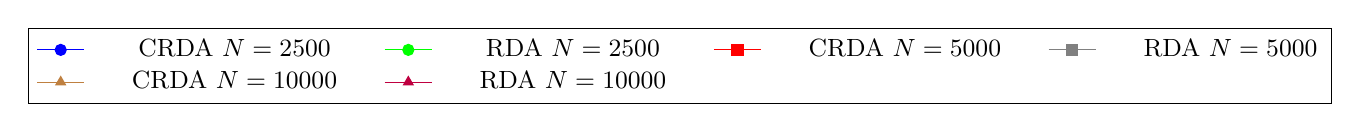
\begin{tikzpicture}
\begin{axis}[
    hide axis,
    xmin=0, xmax=1,
    ymin=0, ymax=1,
    legend columns=4,
    legend style={
        draw,
        at={(0.5,0)},
        anchor=north,
        column sep=1.5em,
        font=\small
    },
]
\addlegendimage{blue, solid, mark=*}
\addlegendentry{CRDA $N = 2500$}
\addlegendimage{rdaN2500}
\addlegendentry{RDA $N = 2500$}

\addlegendimage{red, solid, mark=square*}
\addlegendentry{CRDA $N = 5000$}
\addlegendimage{rdaN5000}
\addlegendentry{RDA $N = 5000$}

\addlegendimage{brown, solid, mark=triangle*}
\addlegendentry{CRDA $N = 10000$}
\addlegendimage{rdaN10000}
\addlegendentry{RDA $N = 10000$}

% \addlegendimage{black, solid, mark=x}
% \addlegendentry{CRDA $N = 100000$}
% \addlegendimage{rdaN100000}
% \addlegendentry{RDA $N = 100000$}
\end{axis}
\end{tikzpicture}
\vspace{0.5cm}

% ===================== ONE: eps = 0.05 =====================
\begin{minipage}[t]{0.33\textwidth}
\centering
\begin{tikzpicture}
\begin{axis}[
    name=mainaxis,
    width=\linewidth,
    height=4.5cm,
    xlabel={$k_2$},
    ylabel={$k_1$},
    title={$\epsilon = 0.05, k = 16$},
    grid=major,
    xmode=log,
    ymode=log,
    mark repeat=20,
]
\addplot table [x=k2,y=k1,col sep=comma,trim cells=true] {estimates_k_16_eps5_N2500.csv};
\addplot table [x=k2,y=k1,col sep=comma] {estimates_k_16_eps5_N5000.csv};
\addplot table [x=k2,y=k1,col sep=comma] {estimates_k_16_eps5_N10000.csv};
\addplot [rdaN2500, smooth] table [x=k2,y=k1,col sep=comma] {estimates_data_eps5_N2500.csv};
\addplot [rdaN5000, smooth] table [x=k2,y=k1,col sep=comma] {estimates_data_eps5_N5000.csv};
\addplot [rdaN10000, smooth] table [x=k2,y=k1,col sep=comma] {estimates_data_eps5_N10000.csv};
% \addplot table [x=k2,y=k1,col sep=comma] {estimates_k_16_eps5_N100000.csv};
\end{axis}

% \begin{axis}[
%     at={(mainaxis.south west)},
%     anchor=south west,
%     width=\linewidth,
%     height=4.5cm,
%     xmode=log,
%     ymode=log,
%     axis lines=none,
%     ticks=none,
% ]
% \addplot [rdaN2500, smooth] table [x=k2,y=k1,col sep=comma] {estimates_data_eps5_N2500.csv};
% \addplot [rdaN5000, smooth] table [x=k2,y=k1,col sep=comma] {estimates_data_eps5_N5000.csv};
% \addplot [rdaN10000, smooth] table [x=k2,y=k1,col sep=comma] {estimates_data_eps5_N10000.csv};
% \addplot [rdaN100000, smooth] table [x=k2,y=k1,col sep=comma] {estimates_data_eps5_N100000.csv};
% \end{axis}
\end{tikzpicture}
\end{minipage}%
\hfill
% ===================== TWO: eps = 0.10 =====================
\begin{minipage}[t]{0.33\textwidth}
\centering
\begin{tikzpicture}
\begin{axis}[
    width=\linewidth,
    height=4.5cm,
    xlabel={$k_2$},
    ylabel={$Data\ Duplication$},
    title={$\epsilon = 0.05, k = 16$},
    grid=major,
    xmode=log,
    ymode=log,
    mark repeat=20,
]
\addplot table [x=k2,y=data_duplication,col sep=comma] {estimates_k_16_eps5_N2500.csv};
\addplot table [x=k2,y=data_duplication,col sep=comma] {estimates_k_16_eps5_N5000.csv};
\addplot table [x=k2,y=data_duplication,col sep=comma] {estimates_k_16_eps5_N10000.csv};
\addplot [rdaN2500, smooth] table [x=k2,y=data_duplication,col sep=comma] {estimates_data_eps5_N2500.csv};
\addplot [rdaN5000, smooth] table [x=k2,y=data_duplication,col sep=comma] {estimates_data_eps5_N5000.csv};
\addplot [rdaN10000, smooth] table [x=k2,y=data_duplication,col sep=comma] {estimates_data_eps5_N10000.csv};
% \addplot table [x=k2,y=data_duplication,col sep=comma] {estimates_k_16_eps5_N100000.csv};
\end{axis}

% \begin{axis}[
%     at={(mainaxis.south west)},
%     anchor=south west,
%     width=\linewidth,
%     height=4.5cm,
%     xmode=log,
%     ymode=log,
%     axis lines=none,
%     ticks=none,
% ]
% \addplot [rdaN2500, smooth] table [x=k2,y=data_duplication,col sep=comma] {estimates_data_eps5_N2500.csv};
% \addplot [rdaN5000, smooth] table [x=k2,y=data_duplication,col sep=comma] {estimates_data_eps5_N5000.csv};
% \addplot [rdaN10000, smooth] table [x=k2,y=data_duplication,col sep=comma] {estimates_data_eps5_N10000.csv};
% % \addplot [rdaN100000, smooth] table [x=k2,y=data_duplication,col sep=comma] {estimates_data_eps5_N100000.csv};
% \end{axis}
\end{tikzpicture}
\end{minipage}%
\hfill
% ===================== THREE: eps = 0.10 =====================
\begin{minipage}[t]{0.33\textwidth}
\centering
\begin{tikzpicture}
\begin{axis}[
    width=\linewidth,
    height=4.5cm,
    xlabel={$k_2$},
    ylabel={$Store\ Complextity$},
    title={$\epsilon = 0.05, k = 16$},
    grid=major,
    xmode=log,
    ymode=log,
    mark repeat=20,
]
\addplot table [x=k2,y=store_complexity,col sep=comma] {estimates_k_16_eps5_N2500.csv};
\addplot table [x=k2,y=store_complexity,col sep=comma] {estimates_k_16_eps5_N5000.csv};
\addplot table [x=k2,y=store_complexity,col sep=comma] {estimates_k_16_eps5_N10000.csv};
\addplot [rdaN2500, smooth] table [x=k2,y=store_complexity,col sep=comma] {estimates_data_eps5_N2500.csv};
\addplot [rdaN5000, smooth] table [x=k2,y=store_complexity,col sep=comma] {estimates_data_eps5_N5000.csv};
\addplot [rdaN10000, smooth] table [x=k2,y=store_complexity,col sep=comma] {estimates_data_eps5_N10000.csv};
% \addplot table [x=k2,y=store_complexity,col sep=comma] {estimates_k_16_eps5_N100000.csv};
\end{axis}

% \begin{axis}[
%     at={(mainaxis.south west)},
%     anchor=south west, c.    
%     height=4.5cm,
%     xmode=log,
%     ymode=log,
%     axis lines=none,
%     ticks=none,
% ]

% \addplot [rdaN100000, smooth] table [x=k2,y=store_complexity,col sep=comma] {estimates_data_eps5_N100000.csv};
% \end{axis}
\end{tikzpicture}
\end{minipage}

\vspace{0.5cm}

% ===================== ONE: eps = 0.05 =====================
\begin{minipage}[t]{0.33\textwidth}
\centering
\begin{tikzpicture}
\begin{axis}[
    name=mainaxis,
    width=\linewidth,
    height=4.5cm,
    xlabel={$k_2$},
    ylabel={$k_1$},
    title={$\epsilon = 0.1, k = 16$},
    grid=major,
    xmode=log,
    ymode=log,
    mark repeat=20,
]
\addplot table [x=k2,y=k1,col sep=comma,trim cells=true] {estimates_k_16_eps10_N2500.csv};
\addplot table [x=k2,y=k1,col sep=comma] {estimates_k_16_eps10_N5000.csv};
\addplot table [x=k2,y=k1,col sep=comma] {estimates_k_16_eps10_N10000.csv};
\addplot [rdaN2500, smooth] table [x=k2,y=k1,col sep=comma] {estimates_data_eps10_N2500.csv};
\addplot [rdaN5000, smooth] table [x=k2,y=k1,col sep=comma] {estimates_data_eps10_N5000.csv};
\addplot [rdaN10000, smooth] table [x=k2,y=k1,col sep=comma] {estimates_data_eps10_N10000.csv};
% \addplot table [x=k2,y=k1,col sep=comma] {estimates_k_16_eps10_N100000.csv};
\end{axis}

% \begin{axis}[
%     at={(mainaxis.south west)},
%     anchor=south west,
%     width=\linewidth,
%     height=4.5cm,
%     xmode=log,
%     ymode=log,
%     axis lines=none,
%     ticks=none,
% ]
% \addplot [rdaN2500, smooth] table [x=k2,y=k1,col sep=comma] {estimates_data_eps10_N2500.csv};
% \addplot [rdaN5000, smooth] table [x=k2,y=k1,col sep=comma] {estimates_data_eps10_N5000.csv};
% \addplot [rdaN10000, smooth] table [x=k2,y=k1,col sep=comma] {estimates_data_eps10_N10000.csv};
% \addplot [rdaN100000, smooth] table [x=k2,y=k1,col sep=comma] {estimates_data_eps10_N100000.csv};
% \end{axis}
\end{tikzpicture}
\end{minipage}%
\hfill
% ===================== TWO: eps = 0.10 =====================
\begin{minipage}[t]{0.33\textwidth}
\centering
\begin{tikzpicture}
\begin{axis}[
    width=\linewidth,
    height=4.5cm,
    xlabel={$k_2$},
    ylabel={$Data\ Duplication$},
    title={$\epsilon = 0.1, k = 16$},
    grid=major,
    xmode=log,
    ymode=log,
    mark repeat=20,
]
\addplot table [x=k2,y=data_duplication,col sep=comma] {estimates_k_16_eps10_N2500.csv};
\addplot table [x=k2,y=data_duplication,col sep=comma] {estimates_k_16_eps10_N5000.csv};
\addplot table [x=k2,y=data_duplication,col sep=comma] {estimates_k_16_eps10_N10000.csv};
\addplot [rdaN2500, smooth] table [x=k2,y=data_duplication,col sep=comma] {estimates_data_eps10_N2500.csv};
\addplot [rdaN5000, smooth] table [x=k2,y=data_duplication,col sep=comma] {estimates_data_eps10_N5000.csv};
\addplot [rdaN10000, smooth] table [x=k2,y=data_duplication,col sep=comma] {estimates_data_eps10_N10000.csv};
% \addplot table [x=k2,y=data_duplication,col sep=comma] {estimates_k_16_eps10_N100000.csv};
\end{axis}

% \begin{axis}[
%     at={(mainaxis.south west)},
%     anchor=south west,
%     width=\linewidth,
%     height=4.5cm,
%     xmode=log,
%     ymode=log,
%     axis lines=none,
%     ticks=none,
% ]
% \addplot [rdaN2500, smooth] table [x=k2,y=data_duplication,col sep=comma] {estimates_data_eps10_N2500.csv};
% \addplot [rdaN5000, smooth] table [x=k2,y=data_duplication,col sep=comma] {estimates_data_eps10_N5000.csv};
% \addplot [rdaN10000, smooth] table [x=k2,y=data_duplication,col sep=comma] {estimates_data_eps10_N10000.csv};
% % \addplot [rdaN100000, smooth] table [x=k2,y=data_duplication,col sep=comma] {estimates_data_eps10_N100000.csv};
% \end{axis}
\end{tikzpicture}
\end{minipage}%
\hfill
% ===================== THREE: eps = 0.10 =====================
\begin{minipage}[t]{0.33\textwidth}
\centering
\begin{tikzpicture}
\begin{axis}[
    width=\linewidth,
    height=4.5cm,
    xlabel={$k_2$},
    ylabel={$Store\ Complextity$},
    title={$\epsilon = 0.1, k = 16$},
    grid=major,
    xmode=log,
    ymode=log,
    mark repeat=20,
]
\addplot table [x=k2,y=store_complexity,col sep=comma] {estimates_k_16_eps10_N2500.csv};
\addplot table [x=k2,y=store_complexity,col sep=comma] {estimates_k_16_eps10_N5000.csv};
\addplot table [x=k2,y=store_complexity,col sep=comma] {estimates_k_16_eps10_N10000.csv};
\addplot [rdaN2500, smooth] table [x=k2,y=store_complexity,col sep=comma] {estimates_data_eps10_N2500.csv};
\addplot [rdaN5000, smooth] table [x=k2,y=store_complexity,col sep=comma] {estimates_data_eps10_N5000.csv};
\addplot [rdaN10000, smooth] table [x=k2,y=store_complexity,col sep=comma] {estimates_data_eps10_N10000.csv};
% \addplot table [x=k2,y=store_complexity,col sep=comma] {estimates_k_16_eps10_N100000.csv};
\end{axis}

% \begin{axis}[
%     at={(mainaxis.south west)},
%     anchor=south west, c.    
%     height=4.5cm,
%     xmode=log,
%     ymode=log,
%     axis lines=none,
%     ticks=none,
% ]

% \addplot [rdaN100000, smooth] table [x=k2,y=store_complexity,col sep=comma] {estimates_data_eps10_N100000.csv};
% \end{axis}
\end{tikzpicture}
\end{minipage}

\caption{(left) $k_1$ vs. $k_2$, (middle) data duplication vs. $k_2$, and (right) storage complexity vs. $k_2$, comparing RobustCDA and RDA across $N \in \{2500, 5000, 10000\}$.}
\end{figure*}

\end{document}
